\documentclass[12pt, spanish]{report}
\usepackage[spanish]{babel}
\usepackage[utf8]{inputenc}
\usepackage[document]{ragged2e}

\usepackage{graphicx}
\graphicspath{{images/}} % Directorio de las imágenes

%%%%%%%%%%%%%%%%%%%%%%%%%%%%%%%%%%%%%%%%%%%%%%%%%%%%%%%%%%%%%%%%%%%%%%%%%%%%%%%%%%%% 
%Bibliografía
%%%%%%%%%%%%%%%%%%%%%%%%%%%%%%%%%%%%%%%%%%%%%%%%%%%%%%%%%%%%%%%%%%%%%%%%%%%%%%%%%%%%

\usepackage{cite} % Paquete para citas bibliográficas
\usepackage{hyperref} % Paquete para crear hipervínculo 
\usepackage{url} % Paquete para url de bibliografía online

\makeatletter
\def\bstctlcite{\@ifnextchar[{\@bstctlcite}{\@bstctlcite[@auxout]}}
\def\@bstctlcite[#1]#2{\@bsphack
	\@for\@citeb:=#2\do{%
		\edef\@citeb{\expandafter\@firstofone\@citeb}%
		\if@filesw\immediate\write\csname #1\endcsname{\string\citation{\@citeb}}\fi}%
	\@esphack}
\makeatother

%%%%%%%%%%%%%%%%%%%%%%%%%%%%%%%%%%%%%%%%%%%%%%%%%%%%%%%%%%%%%%%%%%%%%%%%%%%%%%%%%%%% 
%Configuración de la página
%%%%%%%%%%%%%%%%%%%%%%%%%%%%%%%%%%%%%%%%%%%%%%%%%%%%%%%%%%%%%%%%%%%%%%%%%%%%%%%%%%%%

\usepackage{vmargin}
\setpapersize{A4} % Tamaño de la hoja
\setmarginsrb % Márgenes de la hoja
{3cm}       % Margen izquierdo
{2,5cm}     % Margen superior
{3cm}       % Margen derecho
{1,5cm}     % Margen inferior
{0cm}       % Encabezado
{0cm}       % Separación  
{1cm}       % Pie de página
{1cm}       % Separación  

%%%%%%%%%%%%%%%%%%%%%%%%%%%%%%%%%%%%%%%%%%%%%%%%%%%%%%%%%%%%%%%%%%%%%%%%%%%%%%%%%%%% 
%Configuración de las párrafos y fuentes
%%%%%%%%%%%%%%%%%%%%%%%%%%%%%%%%%%%%%%%%%%%%%%%%%%%%%%%%%%%%%%%%%%%%%%%%%%%%%%%%%%%%

% Niveles que acepta
\setcounter{secnumdepth}{3} % Niveles

% Interlineado
\usepackage{indentfirst}
\renewcommand{\baselinestretch}{1.5} % Interlineado

% Formato personalizado de los capítulos
\usepackage{titlesec}
\titleformat{\chapter}[hang] % Formato de capítulos Ej. 1. Lipsum  
{\normalfont\huge\bfseries}{\thechapter.}{16pt}{\Huge} \titlespacing*{\chapter}{0pt}{-50pt}{10pt} % Args[MarginLeft, MarginTop, MarginBottom]

% Tamaño de los títulos de los capítulos y secciones
\usepackage{titlesec}
\newcommand{\chapfnt}{\fontsize{16}{19}} % Tamaño de capítulos
\newcommand{\secfnt}{\fontsize{14}{17}} % Tamaño de secciones
\newcommand{\ssecfnt}{\fontsize{12}{14}} % Tamaño de subsecciones
\newcommand{\itembf}{\item\textbf}
%%%%%%%%%%%%%%%%%%%%%%%%%%%%%%%%%%%%%%%%%%%%%%%%%%%%%%%%%%%%%%%%%%%%%%%%%%%%%%%%%%%% 
%Bibliografía
%%%%%%%%%%%%%%%%%%%%%%%%%%%%%%%%%%%%%%%%%%%%%%%%%%%%%%%%%%%%%%%%%%%%%%%%%%%%%%%%%%%%

\addto\captionsspanish{\renewcommand{\bibname}{Referencias bibliográficas}} % Renombrar el título de la bibliografía

%%%%%%%%%%%%%%%%%%%%%%%%%%%%%%%%%%%%%%%%%%%%%%%%%%%%%%%%%%%%%%%%%%%%%%%%%%%%%%%%%%%% 
%Otros auxiliares
%%%%%%%%%%%%%%%%%%%%%%%%%%%%%%%%%%%%%%%%%%%%%%%%%%%%%%%%%%%%%%%%%%%%%%%%%%%%%%%%%%%%

%\pagenumbering{gobble} % Quitar la paginación
\usepackage{enumitem}
\usepackage[toc,page]{appendix}
\addto\captionsspanish{%
	\renewcommand\appendixname{Anexo}
	\renewcommand\appendixpagename{Anexos}
}

\usepackage{lscape}
\usepackage{listings}
\usepackage{color}

\definecolor{codegreen}{rgb}{0,0.6,0}
\definecolor{codegray}{rgb}{0.5,0.5,0.5}
\definecolor{codepurple}{rgb}{0.58,0,0.82}
\definecolor{backcolour}{rgb}{0.99,0.99,0.99}
\definecolor{codeblue}{rgb}{0,0,0.92}

\lstdefinestyle{mystyle}{
	backgroundcolor=\color{backcolour},   
	commentstyle=\color{codegreen},
	keywordstyle=\color{codeblue},
	numberstyle=\tiny\color{codegray},
	stringstyle=\color{codepurple},
	basicstyle=\footnotesize,
	breakatwhitespace=false,         
	breaklines=true,                 
	captionpos=b,                    
	keepspaces=true,                 
	numbers=left,                    
	numbersep=5pt,                  
	showspaces=false,                
	showstringspaces=false,
	showtabs=false,                  
	tabsize=2
}

\lstset{literate=
	{á}{{\'a}}1 {é}{{\'e}}1 {í}{{\'i}}1 {ó}{{\'o}}1 {ú}{{\'u}}1
	{Á}{{\'A}}1 {É}{{\'E}}1 {Í}{{\'I}}1 {Ó}{{\'O}}1 {Ú}{{\'U}}1
	{à}{{\`a}}1 {è}{{\`e}}1 {ì}{{\`i}}1 {ò}{{\`o}}1 {ù}{{\`u}}1
	{À}{{\`A}}1 {È}{{\'E}}1 {Ì}{{\`I}}1 {Ò}{{\`O}}1 {Ù}{{\`U}}1
	{ä}{{\"a}}1 {ë}{{\"e}}1 {ï}{{\"i}}1 {ö}{{\"o}}1 {ü}{{\"u}}1
	{Ä}{{\"A}}1 {Ë}{{\"E}}1 {Ï}{{\"I}}1 {Ö}{{\"O}}1 {Ü}{{\"U}}1
	{â}{{\^a}}1 {ê}{{\^e}}1 {î}{{\^i}}1 {ô}{{\^o}}1 {û}{{\^u}}1
	{Â}{{\^A}}1 {Ê}{{\^E}}1 {Î}{{\^I}}1 {Ô}{{\^O}}1 {Û}{{\^U}}1
	{œ}{{\oe}}1 {Œ}{{\OE}}1 {æ}{{\ae}}1 {Æ}{{\AE}}1 {ß}{{\ss}}1
	{ű}{{\H{u}}}1 {Ű}{{\H{U}}}1 {ő}{{\H{o}}}1 {Ő}{{\H{O}}}1
	{ç}{{\c c}}1 {Ç}{{\c C}}1 {ø}{{\o}}1 {å}{{\r a}}1 {Å}{{\r A}}1
	{€}{{\euro}}1 {£}{{\pounds}}1 {«}{{\guillemotleft}}1
	{»}{{\guillemotright}}1 {ñ}{{\~n}}1 {Ñ}{{\~N}}1 {¿}{{?`}}1
}

\lstset{style=mystyle}

\usepackage{courier}

\lstset{basicstyle=\footnotesize\ttfamily,breaklines=true}
%%%%%%%%%%%%%%%%%%%%%%%%%%%%%%%%%%%%%%%%%%%%%%%%%%%%%%%%%%%%%%%%%%%%%%%%%%%%%%%%%%%% 
%Documento principal
%%%%%%%%%%%%%%%%%%%%%%%%%%%%%%%%%%%%%%%%%%%%%%%%%%%%%%%%%%%%%%%%%%%%%%%%%%%%%%%%%%%%

\begin{document}
	\bstctlcite{BSTcontrol}
	\begin{titlepage}
		\begin{center}
			
\includegraphics[width=6cm]{images/logo_utp.png}\\
			\vspace{20pt} 			
			
			\begin{Large}
				Facultad de Ingeniería de Sistemas y Electrónica
			\end{Large}		
			
			\begin{large}
				Carrera profesional de Ingeniería de Sistemas
			\end{large}\vspace{100pt}	
			
			\begin{large}
				\textbf{Informe del proyecto final:}
			\end{large}
		
			\begin{Large}
				Detección de Bad Smells y Refactoring\\
				Aplicación Web de Matrículas
			\end{Large}\vspace{50pt} 	
			
			
			\begin{large}
				\textbf{Autor:}\break
				Canaza Tito, Eddy Wilmer
			\end{large}\vspace{20pt}
			
			\begin{large}
				\textbf{Asesor(a):}\break
				Ing. Paola Ana Zevallos Oporto
			\end{large}\vspace{10pt} 
			\vspace{50pt}	
			
			\vfill
			
			\large{Arequipa, abril de 2017}
		\end{center}
	\end{titlepage}
	
	\tableofcontents
	
	\setlength{\parskip}{0.6em}
	\begin{justify}
	\chapter{Introducción}
	\section{Planteamiento del Problema}




\setlength{\parskip}{0em}
\section{Objetivos}

\subsection{General}
Incrementar el nivel de mantenibilidad de la Aplicación Web de Matrículas a través de Refactoring

\subsection{Específicos}
\begin{itemize}
    \item Investigar técnicas de Refactoring
    \item Estudiar la Aplicación Web de Matrículas
    \item Aplicar técnicas de Refactoring 
    \item Validar la solución
\end{itemize}




\section{Justificación}

	
	\chapter{Marco teórico}
	\section{Refactoring}
Desde su creación los sistemas de software han sido utilizados, probados
e incluso modificados. A lo largo de este período el software y los seres humanos
han interactuado entre sí en forma cotidiana, no pudiéndose concebir
la vida actual del hombre sin la presencia de los sistemas informáticos (comunicaciones,
medicina, transporte, etc.). A tal punto que paulatinamente
los procesos de negocio consumen cada vez más información procesada por
los sistemas de software, incluso hasta a ser controlados y guiados por software.
Por ende, las especificaciones y el diseño de estos sistemas requieren
de supuestos acerca de la aplicación dada, del dominio de la aplicación y de
su ámbito operativo, hecho que a su vez se refleja en el software.


\section{La decadencia del Código Fuente}
Lehman \cite{REF02} \cite{REF01} propone una serie de leyes que guían la evolución de los
sistemas de software:


\begin{enumerate}[label=\textbf{\arabic*}.]
	\itembf{Cambio continuo:} Los sistemas deben adaptarse continuamente de
	lo contrario se hacen progresivamente menos satisfactorios. Estas adaptaciones
	son el resultado del cambio en la operación del entorno en el
	cual la aplicación cumple una función.
	\itembf{Complejidad creciente:} A medida que evoluciona un programa,
	su complejidad se incrementa, a menos que se trabaje para mantenerla
	o reducirla. Esta ley implica un tipo de degradación o entropía en la
	estructura del programa. Esto a su vez conlleva a un aumento progresivo
	del esfuerzo de mantenimiento, a menos que se realice algún tipo
	de mantenimiento perfectivo a este respecto.

	\itembf{Autoregulación:} El proceso de evolución el programa se autoregula
	con una distribución de medidas de atributos de producto y procesos
	cercana a la normal.
	\itembf{Conservación de la Estabilidad Organizativa:} La velocidad de
	actividad global efectiva media en un sistema en evolución es invariante
	a lo largo del ciclo de vida del producto.
	\itembf{Conservación de la Familiaridad}: Durante la vida activa de un
	programa en evolución, el contenido de las versiones sucesivas es estadísticamente
	invariante.
	\itembf{Crecimiento Continuo:} El contenido funcional de un programa
	debe incrementarse continuamente para mantener la satisfacción del
	usuario durante su ciclo de vida.
	\itembf{Calidad Decreciente:} Los sistemas serán percibidos como de calidad
	decreciente a menos que se mantengan de manera rigurosa y se adapten
	al entorno operativo cambiante.
\end{enumerate}

\section{Mal olor en el código fuente}
¿Cuándo un sistema de software comienza a tomar mal olor? Un programador
experimentado puede intuir que su programa va camino a oler mal
cuando hay \cite{REF03}:


\begin{enumerate}[label=\textbf{\arabic*}.]
\itembf{Código duplicado:} Se deben eliminar las líneas de código que son exactamente
iguales en varios sitios, o bien eliminar líneas de código muy
parecidas o con estructura similar en varios sitios.
\itembf{Métodos muy largos:} En este caso hay que particionar el código fuente
en trozos y extraerlos para crear métodos más pequeños, que sean más
fáciles de mantener y de reusar.
\itembf{Clases muy grandes:} En estos casos se debería tratar de identificar
qué cosas hace esa clase, ver si realmente todas esas cosas tienen algo
que ver la una con la otra y si no es así, hacer clases más pequeñas, de
forma que cada una trate una de esas cosas. Por ejemplo, si una clase
es una ventana, además realiza cálculos y escribe los resultados en una
base de datos, ya está haciendo demasiadas cosas. Debería haber una
clase que sea la ventana, otra que realice los cálculos y otra que sepa
escribir en base de datos.
\itembf{Métodos que necesitan muchos parámetros:} Suele ser buena solución
hacer una clase que contenga esos parámetros y pasar la clase en vez
de todos los parámetros. Especialmente si esos parámetros suelen tener
que ver unos con otros y suelen ir juntos siempre.
\itembf{Instrucciones Switch-Case:} Normalmente un switch-case se tiene que
repetir en el código en varios sitios, aunque en cada sitio sea para hacer
cosas distintas. Existen formas, usando el polimorfismo, que evitan

tener que realizar esta repetición a lo largo del código fuente, o incluso
evitan tener que ponerlo en algún lado.

\end{enumerate}

Estas y otras pautas dan al programador la idea de que su código fuente
puede ser susceptible a producir mal olor en un corto lapso de tiempo.

Dentro de este panorama casi desolador surge el concepto de refactorización
de código fuente como una técnica que permite mejorar la comprensibilidad,
la claridad, el diseño, la legibilidad y a su vez reducir la cantidad de
errores. En definitiva una técnica para mejorar la calidad del software.

En un principio asociada a la programación orientada a objetos, el concepto
de refactorización fue extendiéndose hacia otros paradigmas de programación,
teniendo en cuenta la gran cantidad de código fuente escrito en los
últimos 50 años de existencia del campo de la informática.

\section{Refactoring}
El primer uso conocido del término refactorización en la literatura se
encuentra publicado en el artículo Refactoring: An Aid in Designing Application
Frameworks and Evolving Object-Oriented Systems por William F.
Opdyke y Ralph E. Johnson \cite{REF04}. La refactorización surge como un intento
de mejorar la producción de software reusable. El desarrollo de software es
un proceso complejo y continuo en el cual un producto transita, a lo largo de
su construcción, por un proceso iterativo (desarrollo espiral, desarrollo por
prototipos, desarrollo de tipo iterativo incremental, otros). El desarrollo de
software re-usable es un proceso aun más complejo pues éste es el resultado
de varias iteraciones de diseño, incluso cuando éste ya ha sido reusado, por
ende los cambios a los que está sujeto, no lo afectan únicamente a él sino
también al software que lo utiliza \cite{REF05}. En base a ello la refactorización surge
como “el proceso en el cual se aplican cambios en un sistema de software de
forma tal que no altere el comportamiento externo del código, mejorando su
estructura interna” \cite{REF03}.

Esta definición, que no deja de ser muy abierta, plantea una serie de cuestiones:
¿En qué consiste el comportamiento externo del software? ¿El área
de aplicabilidad de la refactorización está restringida únicamente a software
reusable? ¿Puede extenderse este concepto a otros productos del proceso de

desarrollo, o es solamente aplicable a código fuente? ¿En qué consiste la estructura
interna? ¿Cuándo, dónde, por qué refactorizar?


\subsection{El comportamiento externo}
Dentro de la definición de refactorización, existe un concepto en el cual
hay que detenerse un segundo: la idea de la preservación del comportamiento
externo del software. Por definición el proceso de refactorización de código
fuente debe preservar el comportamiento del software. Pero ¿qué se entiende
por comportamiento? En la bibliografáa no se encuentra una definición exacta
sobre qué es el comportamiento externo del software. En su tesis Opdyke
\cite{REF05}, sostiene que el conjunto de entrada y el conjunto de salida deben ser
los mismos antes y después de aplicar el proceso de refactorización. Si bien
en la definición de Opdyke los conjuntos de entrada y salida se conservan,
Mens y Tourwé \cite{REF06} agregan que ver la conservación del comportamiento sólo
desde el punto de vista de las entradas/salidas es exiguo, pues existen otros
aspectos dependiendo del dominio que hay que tener en cuenta. Este último
enfoque permite ampliar la definición de comportamiento que debe ser o
no preservado, dependiendo del dominio e incluso a veces dependiendo de las
necesidades del usuario. Mens y Tourwé proponen tipos distintos de dominios:

\begin{itemize}
	\item Software de tiempo real, en el cual los procesos de refactoring deben
	preservar las restricciones temporales. El tiempo es un factor que forma
	parte del comportamiento externo en este caso.
	\item Software embebido, el consumo de memoria en este caso forma parte
	del comportamiento a preservar en aplicaciones pertenecientes a este
	dominio.

\end{itemize}

Existen además otros dominios en los cuales se pueden definir otros aspectos
que hacen al comportamiento externo. En las aplicaciones web, el
contenido puede pasar a formar parte del comportamiento externo o como
se especifica en  el conjunto de nodos y los links de navegación entre los
nodos y el conjunto de operaciones disponibles para el usuario y la semántica
de cada operación, pueden ser considerados comportamiento externo, desde
el punto de vista de la refactorización.
A pesar de los intentos de formalización, no existe una definición formal
de lo que es considerado comportamiento externo del software.


\subsection{Características internas y externas del software}
Otro punto destacable aportado por el trabajo de \cite{REF06} es el efecto de los
procesos de refactorización sobre la calidad del software. El software posee características
que se manifiestan en forma externa y otras que son propias de la
estructura interna del mismo, definidas como características internas. En las
primeras encontramos conceptos como robustez, extensibilidad, performance,
reusabilidad, etc. Entre las características internas nos encontramos con
los conceptos de comprensibilidad, legibilidad, correctitud, redundancia, etc.
Los procesos de refactorización pueden afectar a las características internas:
al aplicar reducción de código redundante, al aplicar cambios de nombres de
métodos o variables. Pero también pueden afectar a factores o características
externas que hacen a la calidad del software, por ejemplo la performance. Si
bien se cree que la refactorización de código fuente afecta negativamente en
cuanto a la performance \cite{REF03}, existen estudios que demuestran lo contrario.
Refactorizaciones tendientes a reemplazar instrucciones if con polimorfismo
mejoran la performance de la aplicación gracias a las optimizaciones que hacen
los compiladores actuales \cite{REF06}.


\section{Beneficios}
Al refactorizar un sistema no se pueden solucionar todos los problemas del mismo. Sin
embargo, es una herramienta valiosa, si se aplica regularmente. El refactoring es una
herramienta que puede, y debe, ser utilizada para diversos fines. Las motivaciones para
realizar un refactoring pueden ser varias. A continuación, \cite{REF07}, discute algunas de ellas.


\begin{enumerate}[label=\textbf{\arabic*}.]
	\itembf{Mejora el diseño de software:} 
	
	Sin refactorización, el diseño del programa decaerá. Los programadores desarrollan nuevos
	requerimientos con la finalidad de alcanzar objetivos a corto plazo o cambios en el sistema
	realizados sin una comprensión completa del diseño del sistema. Este pierde su estructura con
	el transcurso del tiempo y se hace más difícil ver el diseño mediante la lectura del código.
	
	El refactoring es en parte poner orden en el código. La pérdida de la estructura de un sistema
	tiene un efecto acumulativo. Cuanto más difícil es ver el diseño en el código del sistema, más
	difícil es mantenerlo. Un código mal diseñado generalmente toma más líneas para que
	funcione. Reducir la cantidad de código no hará que el sistema funcione más rápido, sin
	embargo, puede hacer una gran diferencia en la modificabilidad del código. Refactorizar
	regularmente ayuda a conservar la estructura del sistema.
	
	\itembf{Hace al software fácil de entender}
	
	El programador escribe código que indica a la computadora qué hacer, y esta, responde
	haciendo exactamente lo que le dice. Hay una brecha entre lo que el programador quiere que
	haga y lo que el código realmente hace \cite{REF03}.
	
	A la hora de programar, es una mala práctica que no se piense en que otro programador o el
	mismo en un futuro tenga que modificar el código. Este es un problema que impacta cuando un
	programador necesita una semana para hacer un cambio que habría tomado sólo una hora si el
	código fuera más entendible.
	
	El refactoring ayuda a hacer el código más legible. Cuando existe código que funciona, pero
	no está muy bien estructurado, un poco de tiempo dedicado a refactorizar puede hacer que sea
	más entendible y rápido de modificar.
	
	Se pueden empezar realizando pequeños refactorings corrigiendo detalles. Como el código
	va quedando más claro, se pueden ver aspectos del diseño que no se podían ver antes. 
	
	\itembf{Ayuda a encontrar errores}
	
	Al ayudar a comprender el código también ayuda a localizar errores puntuales. Al refactorizar
	código se trabaja profundamente en la comprensión de lo que hace el código, y se puede
	volcar ese nuevo entendimiento de nuevo en el código. Tomar como un hábito la refactorización
	permite escribir código robusto de forma más eficiente.

\end{enumerate}

\section{Momentos para refactorizar}
Se recomienda refactorizar todo el tiempo en pequeñas ráfagas. El desarrollador no decide
refactorizar, refactoriza porque quiere hacer algo más, y refactorizando ayuda a preparar el
sistema para el cambio. A continuación,, se discuten algunas guías de cuándo es recomendable
refactorizar.
\begin{enumerate}[label=\textbf{\arabic*}.]
	\itembf{Al agregar una funcionalidad}
	
	El momento más común para refactorizar es cuando se quiere agregar una nueva
	funcionalidad a un sistema. El código puede haber sido escrito por el mismo programador al
	que le toca implementarla o por otro. Al momento de agregarla, el programador ve que si se
	hubiera diseñado el código de otra manera, la implementación sería más fácil. Se debe
	refactorizar el diseño para que el sistema se más fácil de modificar en el futuro y por la tanto el
	proceso de agregar una nueva funcionalidad sea más rápido.

	
	\itembf{Al corregir un error}
	
	Cuando se mira el código al tratar de entenderlo, se refactoriza para ayudar a mejorar la
	comprensión. Este proceso activo de trabajar con el código ayuda a encontrar errores. Si se
	reporta un error en el sistema, es una clara señal de que se necesita una refactorización, ya
	que el código no era lo suficientemente claro para que el desarrollador vea que había un error
	en el área en la que trabajó.

	
	\itembf{Al revisar el código}
	
	Las revisiones de código ayudan a difundir el conocimiento a través de un equipo de
	desarrollo. Los desarrolladores más experimentados pasan conocimiento a otros con menos
	experiencia. También son muy importantes para la escritura de código claro. El código puede
	parecer claro para el desarrollador que lo escribió, pero no para el resto del equipo. Las
	revisiones también dan la oportunidad para que más personas sugieren ideas útiles. 
\end{enumerate}

	
	\chapter{Metodología}
	Para esta etapa del proyecto se detectarán los bad smells del código existente del pro proyecto y se aplicarán técnicas de refactoring e ingeniería para resolverlos.

\section{Revisión de los Shared Layout de las vistas}
\subsection{Librerías de terceros innecesarias}
\begin{itemize}
	\item \textbf{Síntoma:} Existen librerías de terceros procedentes de la plantilla que no se utilizan en ningún momento.
	\item \textbf{Solución:} Revisar que librerías se están usando dentro del proyecto. 
	\item \textbf{Procedimiento:} Se eliminó la carpeta que contenía los elementos de la plantilla, se migraron los paquetes a bower y se reciclo las hojas de estilos. Además, se escribió comentarios indicando la función que cumple cada uno.
\end{itemize}

\begin{lstlisting}[language=html]
@* CSS *@
<!-- Fuentes -->
<!-- Plugins -->
<!-- Bootstrap -->
<link href="~/lib/bootstrap/dist/css/bootstrap.css" rel="stylesheet" /> 
 <!-- Mensajes emergentes -->
<link href="~/lib/toastr/toastr.css" rel="stylesheet" />
<!-- Iconos -->
<!-- Iconos principales -->
<link href="~/lib/fontawesome/css/font-awesome.css" rel="stylesheet" /> 
<!-- Estilos de la aplicacion -->
<!-- Normalizacion de elementos -->
<link href="~/css/components.css" rel="stylesheet" /> 

@* JavaScript *@
<!-- jQuery -->
<script src="~/lib/jquery/dist/jquery.min.js"></script> 
<!-- Bootstrap -->
<script src="~/lib/bootstrap/dist/js/bootstrap.min.js"></script> 
<!-- Waypoints: Trigger para iniciar funcion -->
<script src="~/lib/waypoints/lib/jquery.waypoints.min.js"></script> 
\end{lstlisting}

\subsection{Error en la carga de las vistas}
\begin{itemize}
	\item \textbf{Síntoma:} Las vistas de la aplicación presentan un ligero retardo al cargar la data.
	\item \textbf{Solución:} Revisar las directivas de Angular. 
	\item \textbf{Procedimiento:} Se agregó la directiva ng-cloak
\end{itemize}

\begin{lstlisting}[language=html]
<div class="row" ng-app="app" ng-controller="alumnosController as vm">
	<wait-cursor display-when="vm.isBusy"></wait-cursor>
	<!-- Tabla de visualizacion -->
	<div ... ng-cloak>
		...
	</div>
</div>
\end{lstlisting}

\subsection{Error en la carga de las vistas}
\begin{itemize}
	\item \textbf{Síntoma:} Los archivos javascript de la aplicación están mezclados con los controladores angular.
	\item \textbf{Solución:} Colocar todos los controladores dentro de una carpeta.
	\item \textbf{Procedimiento:} Se creó la carpeta ``angular" para trasladar los controladores y se cambió la ruta de los paquetes en las vistas.
\end{itemize}

\begin{figure}[h]
	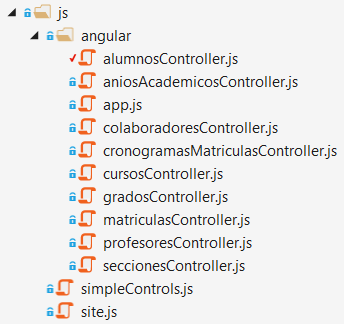
\includegraphics[width=0.5\textwidth]{1.png}
	\centering
\end{figure}

\begin{lstlisting}[language=html]
@section scripts {
	...
	<script src="~/js/angular/app.js"></script>
	<script src="~/js/angular/alumnosController.js"></script>
	...
}
\end{lstlisting}

\subsection{Validación de los nested objects}
\begin{itemize}
	\item \textbf{Síntoma:} El controlador no valida los nested objects.
	\item \textbf{Solución:} Crear una clase que realice este proceso iterativamente.
	\item \textbf{Procedimiento:} Se creó dos clases, una llamada ``CompositeValidationResult" y la otra ``ValidateObjectAttribute" que agregan un atributo a los decoradores de validación del modelo para que puedan usarse en todos los DTO.
\end{itemize}

\begin{figure}[h]
	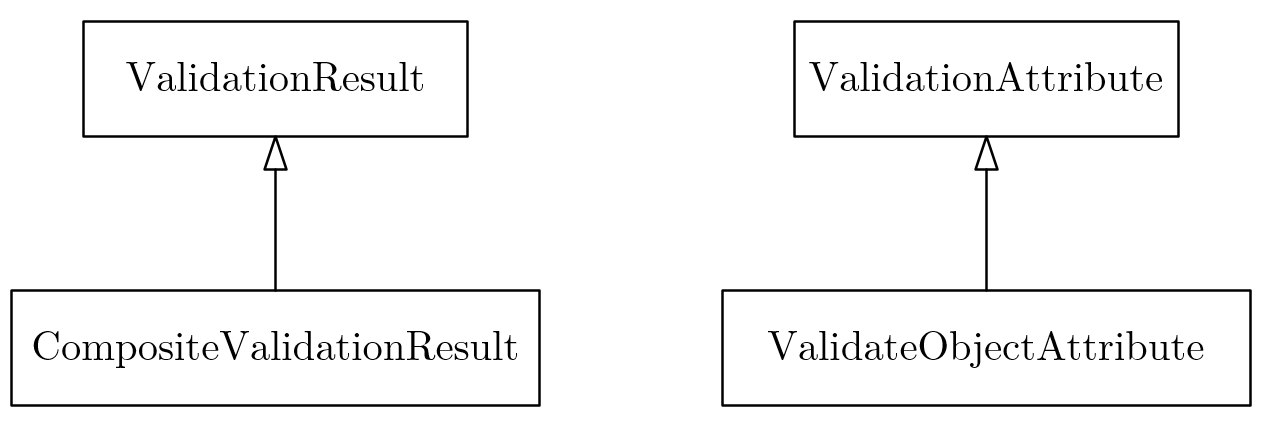
\includegraphics[width=0.7\textwidth]{2.png}
	\centering
\end{figure}

\begin{lstlisting}[language={[Sharp]C}]
public class AlumnoViewModel
{
	...
	[Required, ValidateObject]
	public virtual ApoderadoViewModel Apoderado { get; set; }
	...
}
\end{lstlisting}


	
	\titlespacing*{\chapter}{0pt}{-50pt}{20pt}

	\bibliographystyle{IEEEtran}
	\bibliography{biblio}
	\end{justify}
	
%	\appendix
%	\appendixpage
%	\chapter{Requisitos funcionales}

	
\end{document}
